%%%%%%%%%%%%%%%%%%%%%%%%%%%%%%%%%%%%%%%%%
% Cleese Assignment (For Students)
% LaTeX Template
% Version 2.0 (27/5/2018)
%
% This template originates from:
% http://www.LaTeXTemplates.com
%
% Author:
% Vel (vel@LaTeXTemplates.com)
%
% License:
% CC BY-NC-SA 3.0 (http://creativecommons.org/licenses/by-nc-sa/3.0/)
% 
%%%%%%%%%%%%%%%%%%%%%%%%%%%%%%%%%%%%%%%%%

%----------------------------------------------------------------------------------------
%	PACKAGES AND OTHER DOCUMENT CONFIGURATIONS
%----------------------------------------------------------------------------------------

\documentclass[11pt]{article}
\usepackage{amssymb}
\usepackage{float}  
\usepackage{subcaption}
\usepackage{url}
\input{structure.tex} % Include the file specifying the document structure and custom commands

%----------------------------------------------------------------------------------------
%	ASSIGNMENT INFORMATION
%----------------------------------------------------------------------------------------

% Required
\newcommand{\assignmentQuestionName}{Question} % The word to be used as a prefix to question numbers; example alternatives: Problem, Exercise
\newcommand{\assignmentClass}{Social Networks} % Course/class
\newcommand{\assignmentTitle}{Assignment\ \#3} % Assignment title or name
\newcommand{\assignmentAuthorName}{Ali Dashtbozorg 810104302} % Student name

% Optional (comment lines to remove)
\newcommand{\assignmentClassInstructor}{Dr. Masoud Asadpour 15:00am} % Intructor name/time/description
\newcommand{\assignmentDueDate}{Thursday,\ January\ 4,\ 2026} % Due date

%----------------------------------------------------------------------------------------

\begin{document}

%----------------------------------------------------------------------------------------
%	TITLE PAGE
%----------------------------------------------------------------------------------------

\maketitle % Print the title page

\thispagestyle{empty} % Suppress headers and footers on the title page

\newpage

\tableofcontents % Generates the table of contents
\newpage
\listoffigures   % Generates the list of figures
\newpage


\begin{question}
	\questiontext{Optimizing Structural Balance in a Competitive Network}
	\begin{subquestion}{Using a triadic (triangle-based) analysis, identify the structural patterns that are inconsistent with the definition of strong structural balance. In your answer, specify examples of problematic triangles and describe the sign configuration of their edges.}
		\answer{
		if a complete graph has structural balance we should be able to split it into 2 clusters where inside each cluster the relationship between the nodes is positive but between clusters the relationship between the nodes would be negative the structural patterns that are inconsisitent with the definition of strong balance are when the product of the edges in a triangle are negative so for instance when we have 2 positive edges and one negative and when we have 3 negative edges we consider the triangle unbalanced and if such triangles exist inside a graph the graph is not strongly balanced for instance in the given graph to name a few unbalanced triangles we have:
		\begin{enumerate}
			\item The triangle BCD is unbalanced since CD and CB is positive but DB is negative making the product of signs negative
			\item  The triangle ABD is weakly balanced since all of its edges are negative making the product of signs negative
			\item  The triangle ACD is unbalanced since AC and CD are positive and but AD is negative making the product of signs negative
		\end{enumerate}
		There are many more examples we could make on unbalanced triangles in this graph and we will be discussing why these triangles are created and how to fix them in the next sub-question
		}
	\end{subquestion}
	\begin{subquestion}{The objective is to transform the network into a fully balanced two-faction structure, while minimizing the number of sign changes on edges.}
		\begin{enumerate}
			\item  Determine which edge or edges must change their sign in order for the network to 
			achieve strong structural balance.
			\answer{
			For this question the approach we took was to try and split the graph into 2 different clusters since we know that if a graph is strongly balanced it can be divided into 2 clusters where inside each cluster the relationship between the nodes is positive but between clusters the relationship between the nodes would be negative and in doing so we divided the graph into 2 clusters ${A,B,C}$ and ${D,E,F}$ and we found that the minimum number of edges to be replaced so that the graph achives balance is 2 and the edges are:
			\begin{enumerate}
				\item  AB should change from $-$ to $+$ since the nodes are both inside the same cluster
				\item  CD should change from $+$ to $-$ since the nodes are in different clusters
			\end{enumerate}
			}
			\item After applying these changes, analyze whether the original bipartition of the nodes is preserved or whether a reorganization of the groups is required. If a reorganization occurs, specify the new partition and explain why it is structurally preferable.
			\answer{
			
			}
		\end{enumerate}
	\end{subquestion}
\end{question}
\begin{question}
	\questiontext{Graph Reduction in Large and Irregular Signed Networks}
	
	\begin{subquestion}{Using the standard graph reduction algorithm based on positive connected components, construct the reduced graph $G'$. Clearly specify the vertices of $G'$ (i.e., the supernodes), listing the original nodes contained in each supernode.}
		\answer{
			After applying the graph reduction algorithm, we obtain five supernodes, listed below:
			\begin{itemize}
				\item Supernode $A$ containing nodes $\{6,7,8\}$
				\item Supernode $B$ containing nodes $\{1,2,3,4,5\}$
				\item Supernode $C$ containing nodes $\{14,15,16,17,18\}$
				\item Supernode $D$ containing nodes $\{10,11,12,13\}$
				\item Supernode $E$ containing node $\{9\}$
			\end{itemize}
			
			All edges in the reduced graph are annotated with a negative sign. The edge set of the reduced graph is
			$\{AB, BC, CD, DE, EA, BD\}$.
		}
	\end{subquestion}
	
	\begin{subquestion}{By analyzing the structure of the reduced graph $G'$, determine whether the original network $G$ satisfies the property of strong structural balance. Provide your argument solely based on the examination of cycles present in the graph.}
		\answer{
			A reduced graph violates strong structural balance if it contains a cycle with an odd number of negative edges. In the reduced graph $G'$, the cycle $ABCDEA$ consists of five edges, all of which are negative. Since this cycle has an odd length, the graph is not strongly structurally balanced.
		}
	\end{subquestion}
	
	\begin{subquestion}{The objective is to transform the reduced graph $G'$ into a fully bipolar structure in accordance with the definition of strong structural balance, such that the supernodes are partitioned into exactly two opposing coalitions. Determine the minimum number of edge sign changes (from negative to positive) required to achieve this configuration. Additionally, specify which edge or edges in the reduced graph $G'$ must be modified in order to obtain the desired bipolar partition.}
		\answer{
			To address this question, we work directly with the reduced graph obtained in the previous subquestion. Among all pairs of supernodes, the maximum number of inconsistencies that must be resolved is two. We therefore select supernodes $C$ and $D$ as the initial representatives of the two opposing coalitions.
			
			Supernode $A$ is initially neutral with respect to both coalitions and is temporarily left unassigned. Supernode $B$ is optimally assigned to the coalition containing $D$, since this requires only a single sign change: flipping the sign of edge $4 \to 11$, which corresponds to edge $BD$ in the reduced graph.
			
			With this assignment, supernode $A$ is placed in the coalition containing $C$. For supernode $E$, there are two equally optimal options, each requiring one sign change. These correspond to flipping either edge $7 \to 9$ or $9 \to 10$. For concreteness, we choose to flip the sign of edge $9 \to 10$, which corresponds to edge $ED$ in the reduced graph, thereby assigning $E$ to the coalition containing $D$.
			
			After performing two edge sign changes in total, the network achieves strong structural balance. Although this initially suggests a bipartition of $\{A, C\}$ and $\{B, D, E\}$, the sign changes cause supernodes $B$ and $E$ to merge with $D$. As a result, the reduced graph now consists of three supernodes:
			\begin{itemize}
				\item Supernode $A$ containing nodes $\{6,7,8\}$
				\item Supernode $C$ containing nodes $\{14,15,16,17,18\}$
				\item Supernode $D$ containing nodes $\{1,2,3,4,5,9,10,11,12,13\}$
			\end{itemize}
			
			The final reduced graph contains two negative edges, $AD$ and $CD$, and satisfies the conditions for strong structural balance.
		}
	\end{subquestion}
\end{question}


\begin{question}
	\questiontext{Triadic Closure and Tie Stability in Social Networks}
	\begin{subquestion}{Analyze the structural configuration of node A with respect to the Strong Triadic Closure (STC) principle. Discuss under what changes to the network structure or to the strength of existing ties this configuration could become consistent with the STC principle.}
		\answer{
			To satisfy the STC principle since  A has strong ties to B and C, then there should be an edge (either a strong or weak tie) between B and C. since the question has stated that AD is a local bridge than by definition since A should satisfy STC property the tie is a weak one so no more modifications are needed but if the edge AD wasn't a local bridge and it was strong tie based on STC principle there should have been an edge between B and D (either a strong or weak tie) and also an edge Between C and D  (either a strong or weak tie)
		}
	\end{subquestion}
	\begin{subquestion}{Assume that the network satisfies the Strong Triadic Closure principle. Using a logical argument and the definition of a local bridge, show that the edge (A, D) cannot be a strong tie.
		}
		\answer{
		In this case we will use a proof by contradiction assume for the sake of contradiction that the edge $A \to D$ is a strong tie so by definition of the Strong Triadic Closure principle and edge of any strength should exist between nodes $D$ and $C$ and also an edge of any strength should exist between nodes $D$ and $B$ which contradicts the fact that the edge $A \to D$ is a local bridge therefore, our assumption is false and hence the edge  $A \to D$ is a weak tie
		}
	\end{subquestion}
\end{question}


\begin{question}
	\questiontext{Balance, weak balance and unbalanced networks}
	All of the implementations for this question are provided inside the q4.ipynb file
	\begin{subquestion}{Sign prediction}
		\answer{
			Our algorithm uses a backtracking search to determine if a graph can be "balanced" by assigning positive ($+1$) or negative ($-1$) signs to a specific set of unassigned edges (zero\_edges). It operates by recursively iterating through each unassigned edge and tentatively assigning it a sign, immediately checking if that choice violates the "balance" condition of any associated triangles (triangle\_edges). a triangle is considered balanced if the product of its edge signs is positive (i.e., it contains an even number of negative edges). By performing this "pruning" check early—ensuring a triangle is still valid as soon as an edge within it is signed—the algorithm avoids exploring invalid branches of the search tree. If the algorithm successfully assigns signs to all edges such that every triangle in the set satisfies the balance condition, it returns True; otherwise, it backtracks, resets the edge, and tries a different configuration, returning False if no valid assignment exists.
		}
	\end{subquestion}
	
	\begin{subquestion}{Balance test:}
		\answer{
		Our algorithm evaluates structural balance in a signed graph by identifying "factions" (super-nodes) and analyzing the relationships between them. It begins by isolating all positive edges to determine the graph’s connected components, which represent groups of "friends" that should ideally belong to the same cluster. If any negative edge exists within one of these clusters, it immediately flags a structural contradiction and labels the graph as unbalanced. If internal clusters are consistent, the algorithm constructs a "reduced graph" where each cluster is treated as a single node, connected by the original negative edges. A graph is then declared strongly balanced if this reduced graph is bipartite—meaning all nodes can be split into two opposing camps with no internal conflict—or weakly balanced if there are no internal negative edges but more than two camps exist. Finally, the draw\_clusters function generates a visual map, color-coding nodes by their cluster membership and edges by their sign (blue for positive, red for negative) using a Fruchterman-Reingold layout to reveal the social structure.
	}
	\newpage
\answer{
		\textbf{Network A}
		\textbf{Identified Super-nodes:} 3 factions\\
		\textbf{Result:} Strongly balanced\\
		\textbf{Reason:} The reduced graph is bipartite.
		
		\paragraph{Super-node Assignments}
		\begin{itemize}
			\item Super-node 0 (Size 28): $\{0,2,4,6,9,27,29,1,22,26,15,31,32 \\\hfill
			,33,34,3,7,8,19,24,12,20,5,16,25,11,30,13\}$
			\item Super-node 1 (Size 4): $\{10,14,21,23\}$
			\item Super-node 2 (Size 3): $\{17,18,28\}$
		\end{itemize}
	}
		\begin{figure}[H]
			\centering
			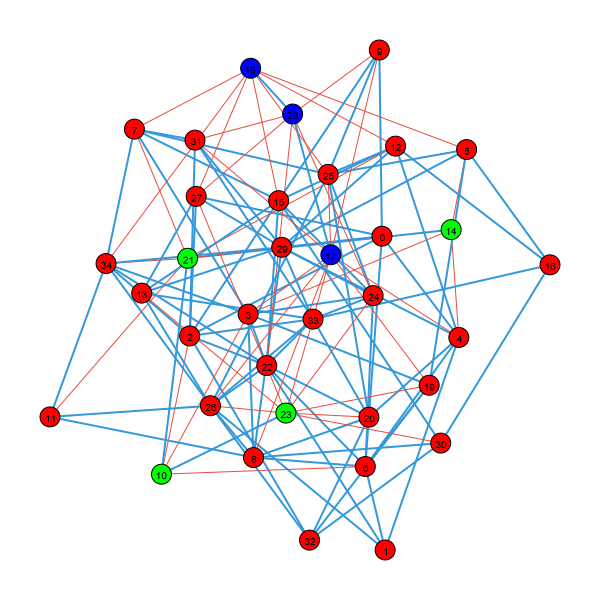
\includegraphics[width=0.6\textwidth]{imgs/clusters_network_a.png}
			\caption{Colored  graph of Network A by supernode assignments}
		\end{figure}
		\newpage
	\answer{
		\textbf{Network B}
		\textbf{Identified Super-nodes:} 3 factions\\
		\textbf{Result:} Unbalanced\\
		\textbf{Reason:} Internal contradiction: nodes 0 and 14 belong to the same super-node but are connected by a negative edge.
		
		\paragraph{Super-node Assignments}
		\begin{itemize}
			\item Super-node 0 (Size 36): $\{0,3,7,9,11,14,21,28,30,34,35,36,1,13,19,32,2\\\hfill
			,5,24,20,26,27,29,31,4,37,18,10,25,33,8,12,17,23,16,22\}$
			\item Super-node 1 (Size 1): $\{6\}$
			\item Super-node 2 (Size 1): $\{15\}$
		\end{itemize}
	}
		\begin{figure}[H]
			\centering
			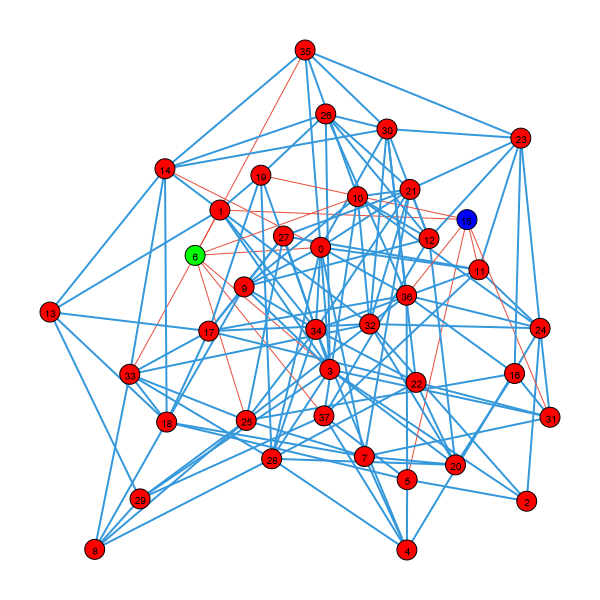
\includegraphics[width=0.6\textwidth]{imgs/clusters_network_b.png}
			\caption{Colored  graph of Network B by supernode assignments}
		\end{figure}
		\newpage
		\answer{
		\textbf{Network C}
		\textbf{Identified Super-nodes:} 3 factions\\
		\textbf{Result:} Unbalanced\\
		\textbf{Reason:} The reduced graph contains an odd cycle.
		
		\paragraph{Super-node Assignments}
		\begin{itemize}
			\item Super-node 0 (Size 15): $\{0,8,9,11,28,31,6,7,21,25,27,4,16,29,30\}$
			\item Super-node 1 (Size 19): $\{23,1,2,3,10,20,22,32,34,18,19,24,5,12,17,26,13,14,15\}$
			\item Super-node 2 (Size 1): $\{33\}$
		\end{itemize}
	}
		\begin{figure}[H]
			\centering
			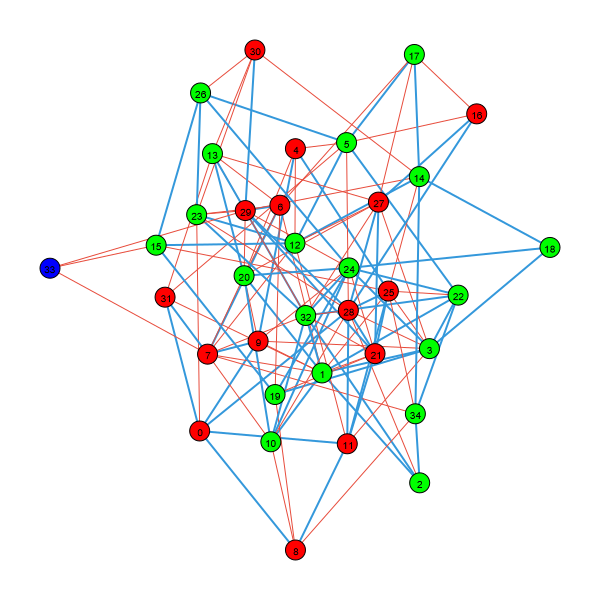
\includegraphics[width=0.6\textwidth]{imgs/clusters_network_c.png}
			\caption{Colored  graph of Network C by supernode assignments}
		\end{figure}
		\newpage
		\answer{
		\textbf{Network D}
		\textbf{Identified Super-nodes:} 5 factions\\
		\textbf{Result:} Unbalanced\\
		\textbf{Reason:} Internal contradiction: nodes 3 and 13 are grouped together but share a negative edge.
		
		\paragraph{Super-node Assignments}
		\begin{itemize}
			\item Super-node 0 (Size 17): $\{0,1,10,11,25,12,15,17,26,7,8,21,16,20,27,18,23\}$
			\item Super-node 1 (Size 1): $\{6\}$
			\item Super-node 2 (Size 1): $\{24\}$
			\item Super-node 3 (Size 1): $\{2\}$
			\item Super-node 4 (Size 9): $\{9,14,28,3,13,19,4,22,5\}$
		\end{itemize}
	}
		\begin{figure}[H]
			\centering
			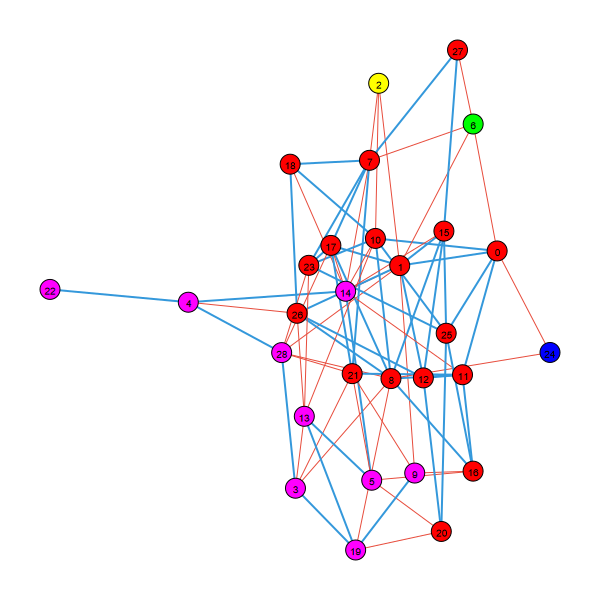
\includegraphics[width=0.6\textwidth]{imgs/clusters_network_d.png}
			\caption{Colored  graph of Network D by supernode assignments}
		\end{figure}
		\newpage
		\answer{
		\textbf{Network E}
		\textbf{Identified Super-nodes:} 2 factions\\
		\textbf{Result:} Unbalanced\\
		\textbf{Reason:} Internal contradiction: nodes 25 and 18 are friends but connected by a negative edge.
	
		\paragraph{Super-node Assignments}
		\begin{itemize}
			\item Super-node 0 (Size 25): $\{0,1,10,22,26,27,2,4,5,8,20,3,12,17\\\hfill
			,21,25,13,29,6,18,23,14,16,15,28\}$
			\item Super-node 1 (Size 5): $\{19,9,24,7,11\}$
		\end{itemize}
	}
		\begin{figure}[H]
			\centering
			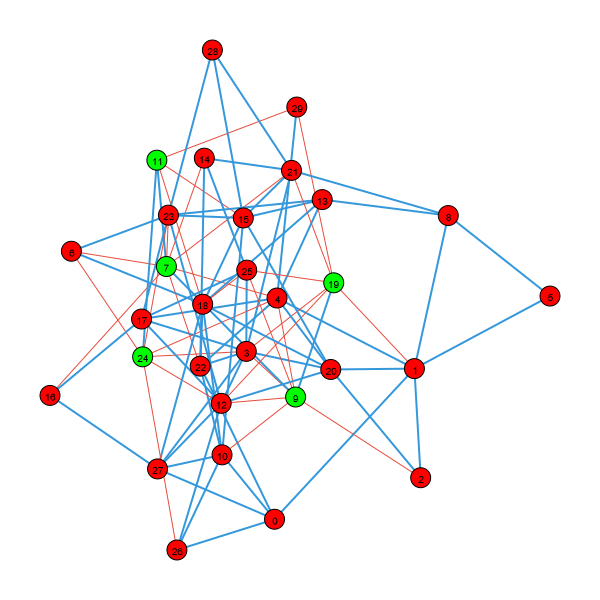
\includegraphics[width=0.6\textwidth]{imgs/clusters_network_e.png}
			\caption{Colored  graph of Network E by supernode assignments}
		\end{figure}
		\newpage
				\answer{
		\textbf{Network F}
		\textbf{Identified Super-nodes:} 3 factions\\
		\textbf{Result:} Strongly balanced\\
		\textbf{Reason:} The reduced graph is bipartite.
		
		\paragraph{Super-node Assignments}
		\begin{itemize}
			\item Super-node 0 (Size 27): $\{0,2,5,7,9,12,21,23,32,1,13,14,17, \\\hfill
			26,28,3,4,19,18,31,11,30,6,20,29,15,33\}$
			\item Super-node 1 (Size 1): $\{16\}$
			\item Super-node 2 (Size 6): $\{27,10,22,24,8,25\}$
		\end{itemize}
	}
		\begin{figure}[H]
			\centering
			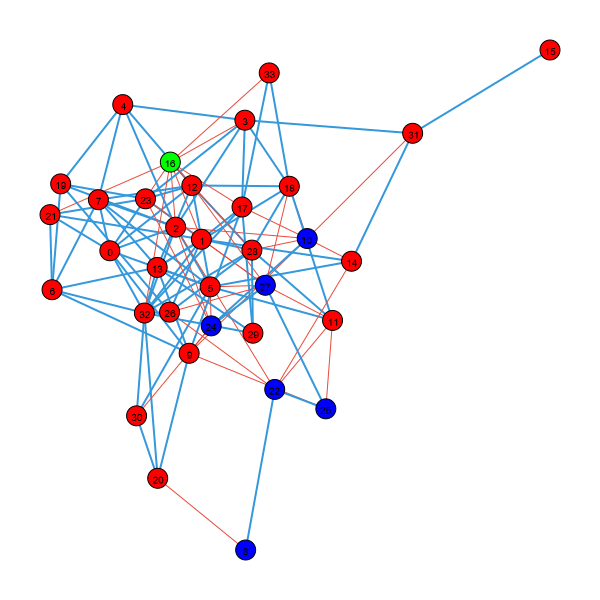
\includegraphics[width=0.6\textwidth]{imgs/clusters_network_f.png}
			\caption{Colored  graph of Network F by supernode assignments}
		\end{figure}
		\newpage
				\answer{
		\textbf{Network G}
		\textbf{Identified Super-nodes:} 3 factions\\
		\textbf{Result:} Unbalanced\\
		\textbf{Reason:} Internal contradiction: nodes 21 and 1 are friends but connected by a negative edge.
		
		\paragraph{Super-node Assignments}
		\begin{itemize}
			\item Super-node 0 (Size 19): $\{0,3,8,17,21,22,1,13,20,2,7,9,16,4,14,5,12,15,19\}$
			\item Super-node 1 (Size 3): $\{10,6,18\}$
			\item Super-node 2 (Size 1): $\{23\}$
		\end{itemize}
	}
		\begin{figure}[H]
			\centering
			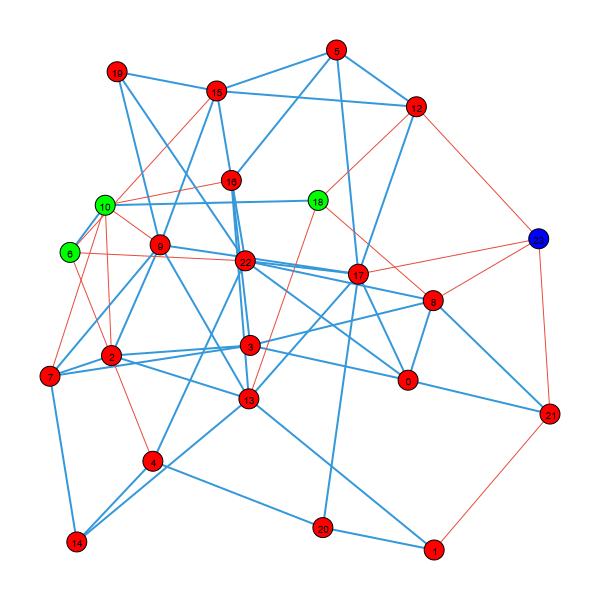
\includegraphics[width=0.6\textwidth]{imgs/clusters_network_g.png}
			\caption{Colored  graph of Network G by supernode assignments}
		\end{figure}
		\newpage
				\answer{
		\textbf{Network H}
		\textbf{Identified Super-nodes:} 5 factions\\
		\textbf{Result:} Strongly balanced\\
		\textbf{Reason:} The reduced graph is bipartite.
		
		\paragraph{Super-node Assignments}
		\begin{itemize}
			\item Super-node 0 (Size 25): $\{0,1,13,21,22,8,19,24,25,2,23,3,11,17,\\\hfill
			4,12,20,28,18,16,10,27,29,14,15\}$
			\item Super-node 1 (Size 2): $\{26,7\}$
			\item Super-node 2 (Size 1): $\{6\}$
			\item Super-node 3 (Size 1): $\{9\}$
			\item Super-node 4 (Size 1): $\{5\}$
		\end{itemize}
	}
		\begin{figure}[H]
			\centering
			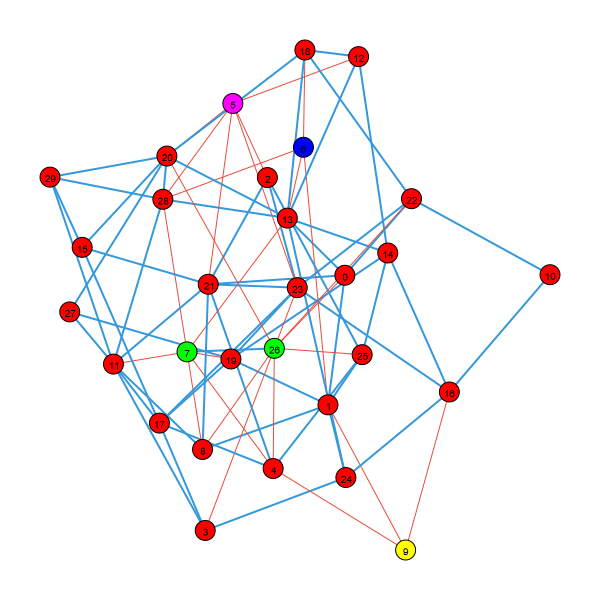
\includegraphics[width=0.6\textwidth]{imgs/clusters_network_h.png}
			\caption{Colored  graph of Network H by supernode assignments}
		\end{figure}
		\newpage
	\end{subquestion}
	\begin{subquestion}{Clusterability}
		\answer{
		We used the same method as the last question but here we didn't enforce bipartitness and allowed weakly balanced networks
		}
		\answer{
		\textbf{Network A}
		\textbf{Identified Super-nodes:} 3 factions \\
		\textbf{Result:} Strongly balanced\\
		\textbf{Reason:} The reduced graph is bipartite. Since every strongly balanced graph is also weakly balanced, this network satisfies the conditions for weak structural balance. Moreover, because the reduced graph admits a bipartition into two opposing groups, clusters 2 and 0 can be merged. By the definition of strong structural balance for incomplete networks, this results in a strongly balanced network.

		
		\paragraph{Super-node Assignments}
		\begin{itemize}
			\item Super-node 0 (Size 5): $\{4,7,12,2,0\}$
			\item Super-node 1 (Size 5): $\{1,3,13,11,10\}$
			\item Super-node 2 (Size 4): $\{9,5,8,6\}$
		\end{itemize}
	}
		\begin{figure}[H]
			\centering
			
\includegraphics[width=0.6\textwidth]{imgs/q4_partc_images/clusters_network_a.png}
			\caption{Colored graph of Network A by cluster assignment}
		\end{figure}
		\newpage
		\answer{
		\textbf{Network B}
		\textbf{Identified Super-nodes:} 4 factions\\
		\textbf{Result:} Weakly balanced\\
		\textbf{Reason:} No inner-cluster negative edges are present, but the reduced graph is not bipartite.
		
		\paragraph{Super-node Assignments}
		\begin{itemize}
			\item Super-node 0 (Size 5): $\{14,10,9,0,8\}$
			\item Super-node 1 (Size 5): $\{5,15,12,18,2\}$
			\item Super-node 2 (Size 5): $\{7,6,13,17,3\}$
			\item Super-node 3 (Size 5): $\{19,1,11,16,4\}$
		\end{itemize}
	}
		\begin{figure}[H]
			\centering
			
\includegraphics[width=0.6\textwidth]{imgs/q4_partc_images/clusters_network_b.png}
			\caption{Colored graph of Network B by cluster assignment}
		\end{figure}
		\newpage
		\answer{		
		\textbf{Network C}
		\textbf{Identified Super-nodes:} 4 factions\\
		\textbf{Result:} Weakly balanced\\
		\textbf{Reason:} No inner-cluster negative edges are present, but the reduced graph is not bipartite.
		
		\paragraph{Super-node Assignments}
		\begin{itemize}
			\item Super-node 0 (Size 8): $\{10,13,29,19,7,21,11,16\}$
			\item Super-node 1 (Size 8): $\{1,25,14,15,20,17,24,26\}$
			\item Super-node 2 (Size 7): $\{5,18,8,27,3,28,22\}$
			\item Super-node 3 (Size 7): $\{4,2,9,12,6,23,0\}$
		\end{itemize}
	}
		\begin{figure}[H]
			\centering
			
\includegraphics[width=0.6\textwidth]{imgs/q4_partc_images/clusters_network_c.png}
			\caption{Colored graph of Network C by cluster assignment}
		\end{figure}
		\newpage
		\answer{
		\textbf{Network D}
		\textbf{Identified Super-nodes:} 6 factions\\
		\textbf{Result:} Weakly balanced\\
		\textbf{Reason:} No inner-cluster negative edges are present, but the reduced graph is not bipartite.
		
		\paragraph{Super-node Assignments}
		\begin{itemize}
			\item Super-node 0 (Size 7): $\{33,4,7,12,14,39,0\}$
			\item Super-node 1 (Size 7): $\{34,1,31,35,6,19,29\}$
			\item Super-node 2 (Size 7): $\{16,17,21,2,36,15,8\}$
			\item Super-node 3 (Size 7): $\{24,27,37,20,28,9,5\}$
			\item Super-node 4 (Size 6): $\{32,38,3,26,11,13\}$
			\item Super-node 5 (Size 6): $\{10,18,23,30,22,25\}$
		\end{itemize}
	}
		\begin{figure}[H]
			\centering
			
\includegraphics[width=0.6\textwidth]{imgs/q4_partc_images/clusters_network_d.png}
			\caption{Colored graph of Network D by cluster assignment}
		\end{figure}
		\newpage
		\answer{
		\textbf{Network E}
		\textbf{Identified Super-nodes:} 8 factions\\
		\textbf{Result:} Weakly balanced\\
		\textbf{Reason:} No inner-cluster negative edges are present, but the reduced graph is not bipartite.
		
		\paragraph{Super-node Assignments}
		\begin{itemize}
			\item Super-node 0 (Size 8): $\{48,26,9,12,18,0,54,46\}$
			\item Super-node 1 (Size 8): $\{16,50,11,58,47,2,27,23\}$
			\item Super-node 2 (Size 8): $\{24,14,21,5,6,32,56,43\}$
			\item Super-node 3 (Size 8): $\{22,42,25,29,52,49,34,31\}$
			\item Super-node 4 (Size 7): $\{19,53,1,8,4,7,13\}$
			\item Super-node 5 (Size 7): $\{35,41,36,3,55,30,10\}$
			\item Super-node 6 (Size 7): $\{28,17,37,39,44,59,33\}$
			\item Super-node 7 (Size 7): $\{57,15,38,45,20,40,51\}$
		\end{itemize}
	}
		\begin{figure}[H]
			\centering
			
\includegraphics[width=0.6\textwidth]{imgs/q4_partc_images/clusters_network_e.png}
			\caption{Colored graph of Network E by cluster assignment}
		\end{figure}
		\newpage
	\end{subquestion}
	\begin{subquestion}{Line Index:}
		\begin{enumerate}
			\item Random clustering:
			\answer{
				The functions \textbf{assign\_random} and \textbf{calculate\_line\_index} perform the random cluster assignment and the line index calculation, respectively. The function \textbf{find\_edge\_between\_clusters} iterates over all combinations of vertices from different clusters and identifies positive and negative edges between them, which aids in the computation of the line index.
			}
			
			\item Heuristic:
			\answer{
				The function \textbf{fix\_clusters} implements a local search optimization procedure to refine social cluster assignments by minimizing structural tension. It iteratively evaluates each node to determine whether moving it to a different cluster would reduce the total cost function, namely the line index. The algorithm continues looping through all nodes until a local optimum is reached, meaning that no single node movement can further reduce the cost. This process ensures that each individual is assigned to the faction in which they experience the fewest social contradictions.
				
				\paragraph{Algorithm Results}
				a sample of the performance of the clustering algorithm is summarized below.
				
				\begin{itemize}
					\item \textbf{Initial random assignment:}
					\begin{itemize}
						\item Positive edges between clusters ($P$): 66
						\item Negative edges within clusters ($N$): 13
						\item Initial line index: 39.5
					\end{itemize}
					
					\item \textbf{After cluster optimization (local search):}
					\begin{itemize}
						\item Positive edges between clusters ($P$): 0
						\item Negative edges within clusters ($N$): 0
						\item Final line index: 0.0
					\end{itemize}
				\end{itemize}
				
				The algorithm achieves a total reduction in frustration of $39.5$, indicating that the final clustering eliminates all structural inconsistencies and attains a fully balanced configuration.
				
			}
		\end{enumerate}
		
	\end{subquestion}
\end{question}


\begin{question}
	\questiontext{Evolution of a School Social Network}
	The order of what questions appear here is not the same as the homework itself
	\begin{subquestion}{Compare smokers and non-smokers: Feature distributions. and Behavioral and attribute evolution over time}
		\answer{
		after running our analysis here is what we achieved
		
		\begin{center}
			\begin{tabular}{lcccccccc}				
				\hline
				\textbf{Day} &  \textbf{Is Smoker} &  \textbf{Connections} & \textbf{Football} & \textbf{Movies}  & \textbf{Clubs} &\textbf{Study}&  \textbf{ Age} &  \textbf{Gender}  \\
				\hline
						1&      False&            0.44&  0.25&  0.43&  0.20&  2.57&  15.86&  0.31 \\
						1&       True&            0.30&  0.55&  0.25&  0.20&  2.60&  16.85&  0.10  \\
						30&      False&            2.45&  0.31&  0.42&  0.24&  2.52&  15.80&  0.30  \\
						30&       True&           13.82&  0.55&  0.58&  0.17&  2.62&  16.72&  0.17  \\
						60&      False&            8.50&  0.48&  0.60&  0.44&  2.56&  15.79&  0.28 \\
						60&       True&           32.88&  0.59&  0.59&  0.21&  1.52&  16.45&  0.26  \\
						90&      False&           21.14&  0.54&  0.66&  0.68&  2.06&  15.90&  0.26  \\
						90&       True&           37.61&  0.71&  0.75&  0.31&  1.08&  16.11&  0.28 \\
				\hline
			\end{tabular}
			\label{table:avg}
		\end{center}
		\begin{enumerate}
			\item \textbf{Social Connections}: our graph on day 1 was very sparse and as time went on did it actually become connected and we see the increase on average Social Connections shown in Table~\ref{table:avg} which reflects this fact but one interesting thing to note is smokers on average had way more social connections throughout the experiment one reason i could think of for this phenomenon is that smokers don't usually smoke alone  they usually have atleast a couple of people around them (smokers or non smokers) and sometimes these hangouts actually do lead to more people becoming smokers
			\item  \textbf{Football}: not much can be said about this alone but considering the fact that smokers had more social connections it is actually pretty logical that they play more football aswell since it's a team sport and well you need a team to play it so more social connection mean more chance you could find people who are willing to play football with you another interesting fact that can be said here is if you look at day 60 and compare it to day 90 there is a sudden spike on there for \textbf{Smokers} and this is due to \textbf{Membership closure} by our calculation from day $60$ to $90$ there were $45$ instances of \textbf{Membership closure} which from that were $25$ smokers added.
			\item \textbf{Movies}: This item is pretty similar to the last item in which people usually go to the movies in groups so having high social connections correlates well with this activity and also the same as football we can see a spike in \textbf{Smokers} who went to the movies this is also due to \textbf{Membership closure} by our calculation from day $60$ to $90$ there were $145$ instances of \textbf{Membership closure} which from that were $28$smokers added.
			\item  \textbf{Clubs}:  This item in particular smokers didn't enjoy as much as the others on the contrary non-smokers had a blast with this activity as this was the highest their activity.
			\item  \textbf{Study}: in this item what we see is that at the start we are close to our average of $3$ but as time goes on first of all we see a downshift of studying so both smoker and non smokers are not studying that much anymore this could have causes unrelated to smoking our test period could have started at the end of the students exams and they didn't have anything to study for for 3 months but if we put that aside what we can clearly see is that non-smokers are far less likely to study compared to smokers and their numbers dropped way faster and reached rock bottom by our analysis nothing major actually happened till day 60 but to start with at first there were 2 people out of the 13 who studied at the max level which were smoking both of these people alongside another persion degraded to level 3 at the start of day 60 also 6 people out of the 8 that left level 4 to go to level 2 were smokers and we can also conclude that most of the people who went from level 2 and 3 to level 1 were also smokers this caused a big \textbf{Membership Closure} of 55 on study level 2 and this trend continued on to day 90 where most of the students are smokers and on level 1  this caused a horrific \textbf{Membership Closure}   of 355 on this level which suddenly dropped the average study of both smokers and non smokers
			\item  \textbf{Age}: from our analysis on this item one thing was certain the smoking problem started from the higher age-group of 18 and spread down as we saw in our calculations at the start 11 out of the 20 smokers were 18 year olds and also 2 out of the most degree-centralized individuals were also 18 and smokers so this lead to an epidemic that spread through all of the years and at the end of day 90 we have a very close margin for smokers between age groups. what we had in this item was \textbf{Focal Closure} as in people with the same age started on becoming friends. based on their age•
			\item  \textbf{Gender}: for this item we really don't have much to say since the average we computed is almost identical to the weighted average of $0.275$ which is the weighted average of the genders so in this case there wasn't any dominance enforced by gender or gender norms here. 
		\end{enumerate}
	}
	\end{subquestion}
	\begin{subquestion}{Compute degree centrality, identify the top 5 most central students at the end of evolution,
			and analyze their role in the network.}
		\answer{
		
		}
	\end{subquestion}
\end{question}

\newpage 
\begin{thebibliography}{9}  % '9' is enough since you have only one reference
	
	\bibitem{chatgpt} 
	ChatGPT, \textit{Chat session used for assignment guidance}, 
	\url{internet was down :( }.
	
\end{thebibliography}
 
%\begin{figure}[H]
	%\centering
	%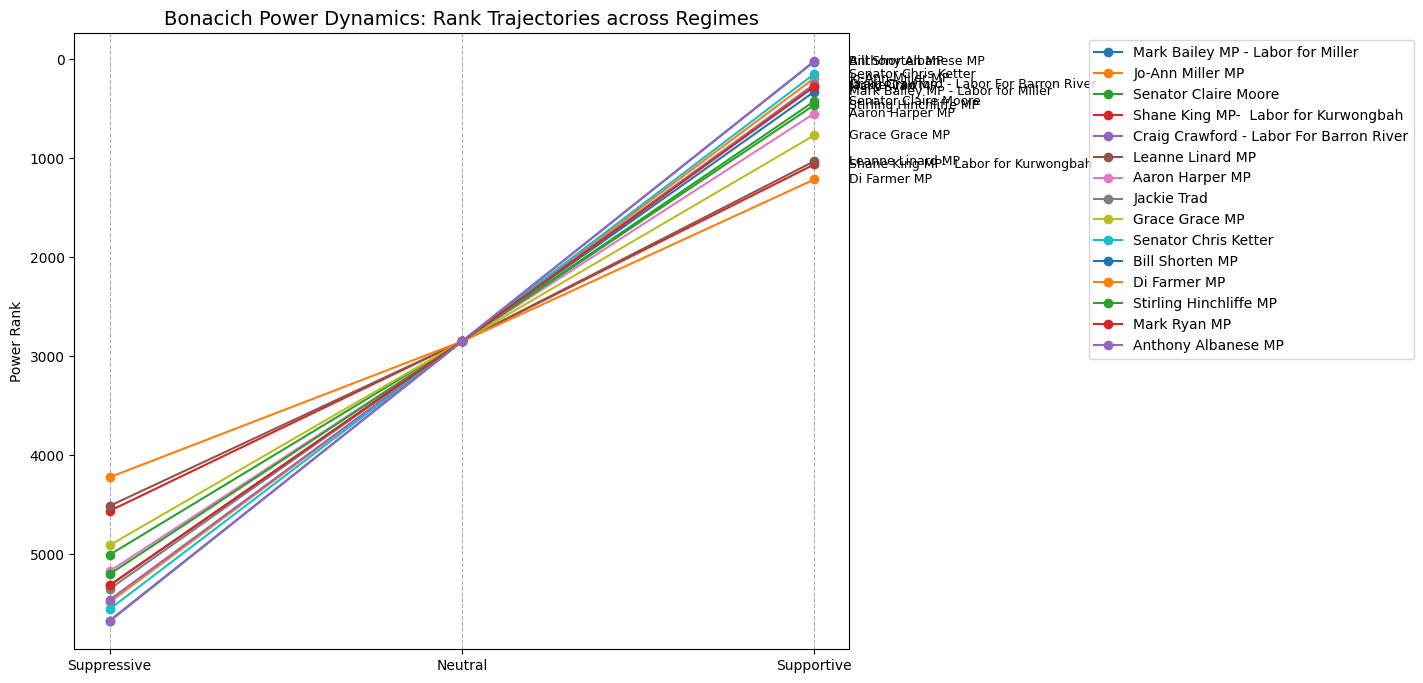
\includegraphics[width=0.85\textwidth,keepaspectratio]{imgs/q4_d_plot.png}
	%\caption{Slope Chart tracking the rank trajectories of key nodes across the neutral, supportive, and suppressive %Bonacich power regimes.}
%	\label{fig:q4_d_plot}
%\end{figure}


\end{document}